% Options for packages loaded elsewhere
\PassOptionsToPackage{unicode}{hyperref}
\PassOptionsToPackage{hyphens}{url}
%
\documentclass[
]{article}
\usepackage{amsmath,amssymb}
\usepackage{iftex}
\ifPDFTeX
  \usepackage[T1]{fontenc}
  \usepackage[utf8]{inputenc}
  \usepackage{textcomp} % provide euro and other symbols
\else % if luatex or xetex
  \usepackage{unicode-math} % this also loads fontspec
  \defaultfontfeatures{Scale=MatchLowercase}
  \defaultfontfeatures[\rmfamily]{Ligatures=TeX,Scale=1}
\fi
\usepackage{lmodern}
\ifPDFTeX\else
  % xetex/luatex font selection
\fi
% Use upquote if available, for straight quotes in verbatim environments
\IfFileExists{upquote.sty}{\usepackage{upquote}}{}
\IfFileExists{microtype.sty}{% use microtype if available
  \usepackage[]{microtype}
  \UseMicrotypeSet[protrusion]{basicmath} % disable protrusion for tt fonts
}{}
\makeatletter
\@ifundefined{KOMAClassName}{% if non-KOMA class
  \IfFileExists{parskip.sty}{%
    \usepackage{parskip}
  }{% else
    \setlength{\parindent}{0pt}
    \setlength{\parskip}{6pt plus 2pt minus 1pt}}
}{% if KOMA class
  \KOMAoptions{parskip=half}}
\makeatother
\usepackage{xcolor}
\usepackage[margin=1in]{geometry}
\usepackage{color}
\usepackage{fancyvrb}
\newcommand{\VerbBar}{|}
\newcommand{\VERB}{\Verb[commandchars=\\\{\}]}
\DefineVerbatimEnvironment{Highlighting}{Verbatim}{commandchars=\\\{\}}
% Add ',fontsize=\small' for more characters per line
\usepackage{framed}
\definecolor{shadecolor}{RGB}{248,248,248}
\newenvironment{Shaded}{\begin{snugshade}}{\end{snugshade}}
\newcommand{\AlertTok}[1]{\textcolor[rgb]{0.94,0.16,0.16}{#1}}
\newcommand{\AnnotationTok}[1]{\textcolor[rgb]{0.56,0.35,0.01}{\textbf{\textit{#1}}}}
\newcommand{\AttributeTok}[1]{\textcolor[rgb]{0.13,0.29,0.53}{#1}}
\newcommand{\BaseNTok}[1]{\textcolor[rgb]{0.00,0.00,0.81}{#1}}
\newcommand{\BuiltInTok}[1]{#1}
\newcommand{\CharTok}[1]{\textcolor[rgb]{0.31,0.60,0.02}{#1}}
\newcommand{\CommentTok}[1]{\textcolor[rgb]{0.56,0.35,0.01}{\textit{#1}}}
\newcommand{\CommentVarTok}[1]{\textcolor[rgb]{0.56,0.35,0.01}{\textbf{\textit{#1}}}}
\newcommand{\ConstantTok}[1]{\textcolor[rgb]{0.56,0.35,0.01}{#1}}
\newcommand{\ControlFlowTok}[1]{\textcolor[rgb]{0.13,0.29,0.53}{\textbf{#1}}}
\newcommand{\DataTypeTok}[1]{\textcolor[rgb]{0.13,0.29,0.53}{#1}}
\newcommand{\DecValTok}[1]{\textcolor[rgb]{0.00,0.00,0.81}{#1}}
\newcommand{\DocumentationTok}[1]{\textcolor[rgb]{0.56,0.35,0.01}{\textbf{\textit{#1}}}}
\newcommand{\ErrorTok}[1]{\textcolor[rgb]{0.64,0.00,0.00}{\textbf{#1}}}
\newcommand{\ExtensionTok}[1]{#1}
\newcommand{\FloatTok}[1]{\textcolor[rgb]{0.00,0.00,0.81}{#1}}
\newcommand{\FunctionTok}[1]{\textcolor[rgb]{0.13,0.29,0.53}{\textbf{#1}}}
\newcommand{\ImportTok}[1]{#1}
\newcommand{\InformationTok}[1]{\textcolor[rgb]{0.56,0.35,0.01}{\textbf{\textit{#1}}}}
\newcommand{\KeywordTok}[1]{\textcolor[rgb]{0.13,0.29,0.53}{\textbf{#1}}}
\newcommand{\NormalTok}[1]{#1}
\newcommand{\OperatorTok}[1]{\textcolor[rgb]{0.81,0.36,0.00}{\textbf{#1}}}
\newcommand{\OtherTok}[1]{\textcolor[rgb]{0.56,0.35,0.01}{#1}}
\newcommand{\PreprocessorTok}[1]{\textcolor[rgb]{0.56,0.35,0.01}{\textit{#1}}}
\newcommand{\RegionMarkerTok}[1]{#1}
\newcommand{\SpecialCharTok}[1]{\textcolor[rgb]{0.81,0.36,0.00}{\textbf{#1}}}
\newcommand{\SpecialStringTok}[1]{\textcolor[rgb]{0.31,0.60,0.02}{#1}}
\newcommand{\StringTok}[1]{\textcolor[rgb]{0.31,0.60,0.02}{#1}}
\newcommand{\VariableTok}[1]{\textcolor[rgb]{0.00,0.00,0.00}{#1}}
\newcommand{\VerbatimStringTok}[1]{\textcolor[rgb]{0.31,0.60,0.02}{#1}}
\newcommand{\WarningTok}[1]{\textcolor[rgb]{0.56,0.35,0.01}{\textbf{\textit{#1}}}}
\usepackage{graphicx}
\makeatletter
\def\maxwidth{\ifdim\Gin@nat@width>\linewidth\linewidth\else\Gin@nat@width\fi}
\def\maxheight{\ifdim\Gin@nat@height>\textheight\textheight\else\Gin@nat@height\fi}
\makeatother
% Scale images if necessary, so that they will not overflow the page
% margins by default, and it is still possible to overwrite the defaults
% using explicit options in \includegraphics[width, height, ...]{}
\setkeys{Gin}{width=\maxwidth,height=\maxheight,keepaspectratio}
% Set default figure placement to htbp
\makeatletter
\def\fps@figure{htbp}
\makeatother
\setlength{\emergencystretch}{3em} % prevent overfull lines
\providecommand{\tightlist}{%
  \setlength{\itemsep}{0pt}\setlength{\parskip}{0pt}}
\setcounter{secnumdepth}{-\maxdimen} % remove section numbering
\ifLuaTeX
  \usepackage{selnolig}  % disable illegal ligatures
\fi
\IfFileExists{bookmark.sty}{\usepackage{bookmark}}{\usepackage{hyperref}}
\IfFileExists{xurl.sty}{\usepackage{xurl}}{} % add URL line breaks if available
\urlstyle{same}
\hypersetup{
  pdftitle={SVD Example},
  hidelinks,
  pdfcreator={LaTeX via pandoc}}

\title{SVD Example}
\author{}
\date{\vspace{-2.5em}2022-08-30}

\begin{document}
\maketitle

This example is from my computing course. These are two handwritten 3's.
We want to align one 3 on top of the other.

\begin{Shaded}
\begin{Highlighting}[]
\NormalTok{X }\OtherTok{\textless{}{-}} \FunctionTok{read.csv}\NormalTok{(}\StringTok{"\textasciitilde{}/Course to teach/Computing/SVD example/X.txt"}\NormalTok{, }\AttributeTok{header=}\ConstantTok{FALSE}\NormalTok{)}

\NormalTok{Y }\OtherTok{\textless{}{-}} \FunctionTok{read.csv}\NormalTok{(}\StringTok{"\textasciitilde{}/Course to teach/Computing/SVD example/Y.txt"}\NormalTok{, }\AttributeTok{header=}\ConstantTok{FALSE}\NormalTok{)}

\NormalTok{X }\OtherTok{\textless{}{-}} \FunctionTok{as.matrix}\NormalTok{(X)}
\NormalTok{Y }\OtherTok{\textless{}{-}} \FunctionTok{as.matrix}\NormalTok{(Y)}

\FunctionTok{plot}\NormalTok{(X, }\AttributeTok{type=}\StringTok{\textquotesingle{}b\textquotesingle{}}\NormalTok{, }\AttributeTok{col=}\DecValTok{1}\NormalTok{, }\AttributeTok{xlim=}\FunctionTok{range}\NormalTok{(}\FunctionTok{c}\NormalTok{(X[,}\DecValTok{1}\NormalTok{], Y[,}\DecValTok{1}\NormalTok{])), }\AttributeTok{ylim=}\FunctionTok{range}\NormalTok{(}\FunctionTok{c}\NormalTok{(X[,}\DecValTok{2}\NormalTok{], Y[,}\DecValTok{2}\NormalTok{])))}
\FunctionTok{points}\NormalTok{(Y, }\AttributeTok{type=}\StringTok{\textquotesingle{}b\textquotesingle{}}\NormalTok{, }\AttributeTok{col=}\DecValTok{2}\NormalTok{)}
\end{Highlighting}
\end{Shaded}

\includegraphics{handwriting-align_files/figure-latex/unnamed-chunk-1-1.pdf}

We first mean center the two images and visualize.

\begin{Shaded}
\begin{Highlighting}[]
\NormalTok{X1 }\OtherTok{\textless{}{-}}\NormalTok{ X }\SpecialCharTok{{-}} \FunctionTok{matrix}\NormalTok{(}\FunctionTok{colMeans}\NormalTok{(X), }\FunctionTok{nrow}\NormalTok{(X), }\DecValTok{2}\NormalTok{, }\AttributeTok{byrow =}\NormalTok{ T)}
\NormalTok{Y1 }\OtherTok{\textless{}{-}}\NormalTok{ Y }\SpecialCharTok{{-}} \FunctionTok{matrix}\NormalTok{(}\FunctionTok{colMeans}\NormalTok{(Y), }\FunctionTok{nrow}\NormalTok{(Y), }\DecValTok{2}\NormalTok{, }\AttributeTok{byrow =}\NormalTok{ T)}



\FunctionTok{plot}\NormalTok{(X1, }\AttributeTok{type=}\StringTok{\textquotesingle{}b\textquotesingle{}}\NormalTok{, }\AttributeTok{col=}\DecValTok{1}\NormalTok{, }\AttributeTok{xlim=}\FunctionTok{range}\NormalTok{(}\FunctionTok{c}\NormalTok{(X1[,}\DecValTok{1}\NormalTok{], Y1[,}\DecValTok{1}\NormalTok{])), }\AttributeTok{ylim=}\FunctionTok{range}\NormalTok{(}\FunctionTok{c}\NormalTok{(X1[,}\DecValTok{2}\NormalTok{], Y1[,}\DecValTok{2}\NormalTok{])))}
\FunctionTok{points}\NormalTok{(Y1, }\AttributeTok{type=}\StringTok{\textquotesingle{}b\textquotesingle{}}\NormalTok{, }\AttributeTok{col=}\DecValTok{2}\NormalTok{)}
\end{Highlighting}
\end{Shaded}

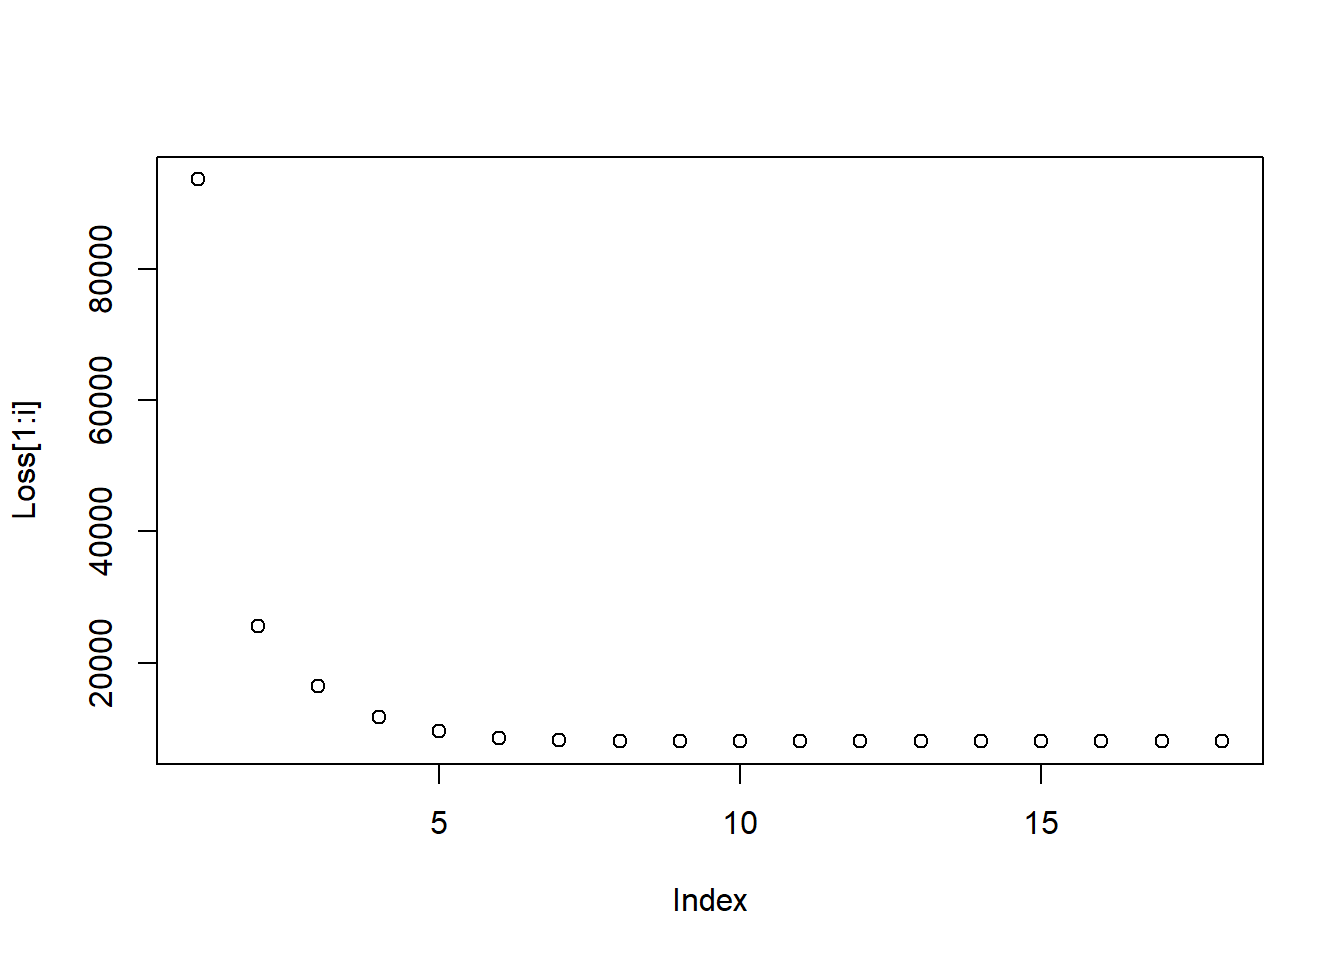
\includegraphics{handwriting-align_files/figure-latex/unnamed-chunk-2-1.pdf}

The difference between images is

\begin{Shaded}
\begin{Highlighting}[]
\FunctionTok{sum}\NormalTok{((X1}\SpecialCharTok{{-}}\NormalTok{Y1)}\SpecialCharTok{\^{}}\DecValTok{2}\NormalTok{)}
\end{Highlighting}
\end{Shaded}

\begin{verbatim}
## [1] 180.9
\end{verbatim}

We now align the two images on top of the other using SVD and also
compute a scalar factor, specifically we solve
\(\min_{\beta,\mathbf{O}}\|X_1-\beta Y_1\mathbf{O}\|_{F}^2\), where
\(\mathbf{O}\) is an orthogonal matrix and \(\beta\) is a scalar.

\begin{Shaded}
\begin{Highlighting}[]
\NormalTok{crosscov }\OtherTok{\textless{}{-}} \FunctionTok{t}\NormalTok{(X1)}\SpecialCharTok{\%*\%}\NormalTok{Y1}
\NormalTok{crosscovSV }\OtherTok{\textless{}{-}} \FunctionTok{svd}\NormalTok{(crosscov) }\CommentTok{\#SVD helps o get crosscov = crosscovSV$u\%*\%diag(crosscovSV$d)\%*\%t(crosscovSV$v)}

\NormalTok{O }\OtherTok{\textless{}{-}}\NormalTok{ crosscovSV}\SpecialCharTok{$}\NormalTok{v }\SpecialCharTok{\%*\%} \FunctionTok{t}\NormalTok{(crosscovSV}\SpecialCharTok{$}\NormalTok{u)}

\NormalTok{Y2 }\OtherTok{\textless{}{-}}\NormalTok{ Y1 }\SpecialCharTok{\%*\%}\NormalTok{ O}

\NormalTok{fit }\OtherTok{\textless{}{-}} \FunctionTok{lm}\NormalTok{(}\FunctionTok{array}\NormalTok{(X1)}\SpecialCharTok{\textasciitilde{}}\FunctionTok{array}\NormalTok{(Y2)}\SpecialCharTok{{-}}\DecValTok{1}\NormalTok{)}
\NormalTok{beta }\OtherTok{\textless{}{-}}\NormalTok{ fit}\SpecialCharTok{$}\NormalTok{coefficients}

\NormalTok{X1hat }\OtherTok{\textless{}{-}}\NormalTok{ beta}\SpecialCharTok{*}\NormalTok{Y2}

\FunctionTok{plot}\NormalTok{(X1, }\AttributeTok{type=}\StringTok{\textquotesingle{}b\textquotesingle{}}\NormalTok{, }\AttributeTok{col=}\DecValTok{1}\NormalTok{, }\AttributeTok{xlim=}\FunctionTok{range}\NormalTok{(}\FunctionTok{c}\NormalTok{(X1[,}\DecValTok{1}\NormalTok{], X1hat[,}\DecValTok{1}\NormalTok{])), }\AttributeTok{ylim=}\FunctionTok{range}\NormalTok{(}\FunctionTok{c}\NormalTok{(X1[,}\DecValTok{2}\NormalTok{], X1hat[,}\DecValTok{2}\NormalTok{])))}
\FunctionTok{points}\NormalTok{(X1hat, }\AttributeTok{type=}\StringTok{\textquotesingle{}b\textquotesingle{}}\NormalTok{, }\AttributeTok{col=}\DecValTok{2}\NormalTok{)}
\end{Highlighting}
\end{Shaded}

\includegraphics{handwriting-align_files/figure-latex/unnamed-chunk-4-1.pdf}

The difference between images after above transformation is

\begin{Shaded}
\begin{Highlighting}[]
\FunctionTok{sum}\NormalTok{((X1}\SpecialCharTok{{-}}\NormalTok{X1hat)}\SpecialCharTok{\^{}}\DecValTok{2}\NormalTok{)}
\end{Highlighting}
\end{Shaded}

\begin{verbatim}
## [1] 166.5321
\end{verbatim}

Note that the error is reduced after the transformation.

\end{document}
